\documentclass[12pt]{article}
\usepackage{amsmath}
\setlength{\jot}{2ex}
\usepackage{mathrsfs}
\usepackage{steinmetz}
\usepackage{graphicx}
\usepackage{wrapfig}
\usepackage{booktabs}
\usepackage[letterpaper, margin=1in]{geometry}
\usepackage{fancyhdr}
\pagestyle{fancy}
\fancyhead[R]{Chapter 10 Problems}
\fancyfoot[C]{\thepage}
\renewcommand{\headrulewidth}{1pt}
\renewcommand{\footrulewidth}{1pt}
\usepackage [autostyle, english = american]{csquotes}
\MakeOuterQuote{"}
\renewcommand{\baselinestretch}{1.0}
\newcommand{\objects}[2]{%
  \leavevmode\vbox{\hbox{#1}\nointerlineskip\hbox{#2}}%
}
\begin{document}
    \section*{Problem 10.8}
    The op amp in the circuit shown is ideal.
    \begin{figure}[h]
        \centering
        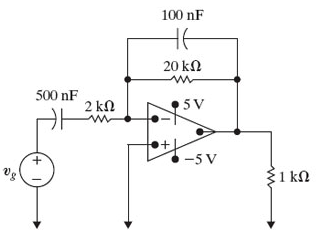
\includegraphics[width=0.4\textwidth]{10.8 Circuit.png}
    \end{figure}
    \\ \textbf{Calculate the average power delivered to the $1\ k \Omega$ resistor
    when $v_{g} = 1.1 \cos (1000t)\ V$.}
    First convert all the elements to the frequency domain and from there the
    equations of ideal op amps can be used to determine the output voltage and
    then the power delivered to the output resistor. \\
    \begin{gather*}
        100\ nF = \frac{-j}{(1000)(100*10^{-9})} = -j 10000 \\
        500\ nF = \frac{-j}{(1000)(500*10^{-9})} = -j 2000 \\
        v_{g} = 1.1 \phase{0^{\circ}} = 1.1\ V
    \end{gather*}
    Since this is an inverting amplifier, the equation for the output voltage is
    given in this case as,
    \[
        v_{o} = -\frac{Z_{f}}{Z_{s}} v_{s}
    .\]
    Here, $R_{f}$ will be equal to the impedance of the $100\ nF$ capacitor and
    the $20\ k \Omega$ resistor in parallel, and $R_{s}$ will be the impedance
    of the $500\ nF$ capacitor with the $2\ k\Omega$ resistor in series.
    \begin{gather*}
        Z_{f} = \frac{(-j 10000)(20*10^{3})}{(-j 10000 + 20*10^{3})} = 4000 - j
        8000\ \Omega \\
        Z_{s} = 2000 - j 2000\ \Omega \\
        v_{o} = - \frac{4000 - j 8000}{2000 - j 2000} (1.1) = -3.3 + j 1.1\ V
    \end{gather*}
    The value attained is the value of the output voltage however, the rms value
    of the voltage is need in order to calculate power.
    \[
        v_{o_{rms}} = \frac{-3.3 + j 1.1}{\sqrt{2}}
    \]
    With this, the power will be equal to,
    \[
        \frac{v_{o_{rms}}^2}{R} = \frac{(-3.3 + j 1.1)^2}{2} \frac{1}{1000} =
        4.84 - j 3.63\ mW
    .\]
    Finally,
    \[
        P = \sqrt{4.84^2 + 3.63^2} = \boxed{6.05\ mW}
    \]
    \section*{Problem 10.10}
    The load impedance in the circuit absorbs $2.5\ kW$ and generates $5\ kVAR$.
    The sinusoidal voltage source develops $7.5\ kW$. Suppose that $R = 20.5\
    \Omega$. \\
    \begin{figure}[h]
        \centering
        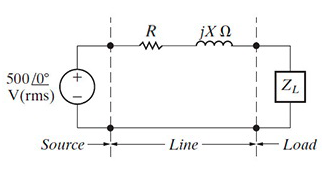
\includegraphics[width=0.5\textwidth]{10.10 Circuit.png}
    \end{figure} \\
    \textbf{Find the minimum and maximum values of inductive line reactance that
    will satisfy these constraints.} \\
    Here, the line loss will be equal to the power absorbed by the resistor
    subtracted from that which is generated by the source,
    \[
        \text{line loss} = 7.5 - 2.5 = 5\ kW
    \]
    The line loss is also equivalent to the current in the branch squared times
    the resistor in the branch, $I^2R$. With this, the current in the branch can
    be found and from there the values of the impedance of the load, $R_{L}$ and
    $X_{L}$, can be determined.
    \begin{gather*}
        I^2 (20.5) = 5000 \\
        I^2 = \frac{5000}{20.5}\ A
    \end{gather*}
    Now, this current squared multiplied by the individual elements within the
    load can give possible values for the resistor and the inductor in said load.
    \begin{gather*}
        I^2 R_{L} = \frac{5000}{20.5} R_{L} = 2500 \\
        I^2 X_{L} = \frac{5000}{20.5} X_{L} = -5000 \\
        R_{L} = 10.25\ \Omega \\
        X_{L} = -20.5\ \Omega
    \end{gather*}
    With this, the equivalent impedance of the circuit can be written as the sum
    of the real and imaginary parts,
    \[
        Z_{eq} = (20.5 + 10. 25) + j (X - 20.5)
    .\]
    Since $V_{s} = 500\ V$, the current in the circuit can be expressed as the
    voltage divided by the magnitude of the equivalent impedance.
    \[
        I = \frac{500}{\sqrt{(30.75)^2 + (X - 20.5)^2}}
    \]
    The value of the current squared is known so this can be solved easily with
    some manipulation.
    \begin{gather*}
        I^2 = \frac{500^2}{(30.75)^2 + (X - 20.5)^2} \\
        \frac{5000}{20.5} = \frac{500^2}{(30.75)^2 + (X - 20.5)^2} \\
        \frac{(30.75)^2(5000)}{20.5} + \frac{5000}{20.5} (X - 20.5)^2 = 500^2 \\
        X = \pm\ \sqrt{\frac{20.5}{5000}\left( 500^2 -
        \frac{(30.75)^2(5000)}{20.5} \right) } + 20.5 \\
        X = \pm\ \sqrt{\frac{(20.5)(500^2)}{5000} - 30.75^2} + 20.5 \\
        \boxed{X_{min} = 11.6\ \Omega \quad X_{max} = 29.4\ \Omega}
    \end{gather*}
    \section*{Problem 10.20}
    Consider the circuit shown. Suppose that $v_{g} = 180 \cos (250 t)$.
    \begin{figure}[h]
        \centering
        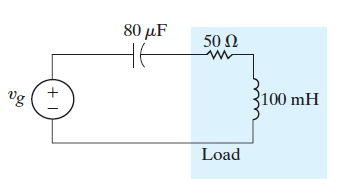
\includegraphics[width=0.5\textwidth]{10.20 Circuit.png}
    \end{figure} \\
    \textbf{Find the average, reactive, and apparent power absorbed by the load
    in the circuit. Use a positive value if the power is absorbed and a negative
    value if the power is delivered.}
    \newpage
    \noindent Converting to the frequency domain,
    \begin{gather*}
        v_{g} = 180 \phase{0^{\circ}} \\
        80\ \mu F = \frac{-j}{(250)(80*10^{-6})} = -j 50 \\
        100\ mH = j (250) (100*10^{-3}) = j 25
    \end{gather*}
    The equivalent impedance can be expressed as,
    \[
        Z_{eq} = 50 - j 25\ \Omega
    ,\]
    and the current as,
    \[
        I = \frac{V}{Z} = \frac{180 \phase{0^{\circ}}}{50 - j 25} = 2.88 + j
        1.44\ A
    .\]
    Using the current, the apparent power can be defined as,
    \begin{gather*}
        S = \frac{1}{2} VI^{*} = \frac{1}{2} (180)(2.88 - j 1.44) \\
        S = 259.2 - j 129.6\ VA \\
        |S| = \sqrt{259.2^2 + 129.6^2} = \boxed{289.79\ VA.}
    \end{gather*}
    The values of average and reactive power can be taken from the apparent
    power as well,
    \[
        \boxed{P = 259.2\ W \quad Q = 129.6\ VAR}
    .\]
    \section*{Problem 10.24}
    Three loads are connected in parallel across a $V_{o} = 350\ V$ (rms) line.
    Load 1 absorbs 16\ kW and 18\ kVAR; Load 2 absorbs 10\ kVA at 0.6 leading;
    Load 3 absorbs 8\ kW at unity power factor.
    \\
    \textbf{Find the impedance that is equivalent to the three parallel loads.}
    \begin{gather*}
        S_1 = 16 + j 18\ kVA \\
        S_2 = 6 - j 8\ kVA \\
        S_3 = 8\ kVA \\
        S_{eq} = (16 + j 18) + (6 - j 8) + 8 = 30 + j 10\ kVA
    \end{gather*}
    Since,
    \begin{gather*}
        S = VI^{*}, \\
        30 + j 10 = 180 I^{*}, \\
        I = 85.7 - j 28.57\ A.
    \end{gather*}
    Now, using the current and the voltage, the impedance can be found.
    \begin{gather*}
        Z = \frac{V}{I} = \frac{350}{85.7 - j 28.57} \\
        \boxed{Z = 3.675 + j 1.225\ \Omega}
    \end{gather*}
    \textbf{Find the power factor of the equivalent load as seen from the line's
    input terminals.}
    \begin{gather*}
        Z = 3.675 + j 1.225 = 3.87 \phase{18.435^{\circ}}\ \Omega \\
        \text{pf} = \cos (18.435^{\circ}) = \boxed{0.9487}
    \end{gather*}
    The power factor is lagging since the angle $\theta_{v} - \theta_{i}$ is
    positive.
    \section*{Problem 10.42}
    The phasor voltage $\textbf{V}_{ab}$ in a circuit is $240 \phase{0^{\circ}}$
    V (rms) when no external load is connected to the terminals $a$ and $b$.
    When a load having an impedance of $80 - j 60\ \Omega$ is connected across
    $a$ and $b$, the value of $\textbf{V}_{ab}$ is $115.2 + j 33.6$ V (rms).
    \subsubsection*{Find the impedance that should be connected across $a$ and
    $b$ for maximum average power transfer.}
    Using the concept of the Thevenin's equivalent voltage and resistance, the
    circuit can be interpreted as a source along with one resistor. This means
    that there are only two impedances connected to the source and since we know
    the voltage when the load is connected, voltage division can be applied to
    determine the value of the Thevenin's resistance.
    \begin{gather*}
        \textbf{V}_{ab} = \frac{Z_{L}}{Z_{TH} + Z_{L}} \textbf{V}_{s} \\
        (115.2 + j 33.6) = \frac{(80 - j 60)}{Z_{TH} + (80 - j 60)} (240
        \phase{0^{\circ}})
    \end{gather*}
    Using this, the value of $Z_{TH}$ can be determined to be,
    \[
        \boxed{Z_{TH} = 40 - j 100\ \Omega}
    \]
    \textbf{Find the maximum average power transferred to the load.}
    \\ For maximum power,
    \begin{gather*}
        Z_{L} = Z_{TH}^{*} \\
        Z_{L} = 40 + j 100\ \Omega
    \end{gather*}
    The combined impedance will simply be a resistance of $80\ \Omega$, meaning
    the current in the circuit is $3\ A$. Since the power will be equal to
    $I^2R$, the maximum power will equal $3^2(40)$.
    \[
        \boxed{P = 360\ W}
    \]
\end{document}
